\documentclass[11pt]{article}
\usepackage[review]{acl}
\usepackage{times}
\usepackage{latexsym}
\usepackage[T1]{fontenc}
\usepackage[utf8]{inputenc}
\usepackage{microtype}
\usepackage{inconsolata}
\usepackage{booktabs}
\usepackage{array}
\usepackage{amsmath}
\usepackage{xurl}
\usepackage{tikz}
\usepackage{pgfplots}
\usepgfplotslibrary{statistics}
\usetikzlibrary{calc,positioning}
\pgfplotsset{compat=1.17}

% Generated by tools/paper_numbers.py from runs/paper-metrics-20261125.json. Do not edit.
\newcommand{\vOneN}{50}
\newcommand{\vOneDistinct}{6}
\newcommand{\vOneLetters}{421}
\newcommand{\vOneLettersMin}{400}
\newcommand{\vOneLettersMed}{423}
\newcommand{\vOneLettersMax}{430}
\newcommand{\vOneWords}{125}
\newcommand{\vOneExact}{100}
\newcommand{\vOneExactCheck}{50}
\newcommand{\vOneShort}{29.8}
\newcommand{\vOneWordLen}{3.37}
\newcommand{\vOneTTR}{0.80}
\newcommand{\vOneBigrams}{96.8}
\newcommand{\vOneSentWords}{124.7}
\newcommand{\vOneLM}{\ensuremath{-9.12}}
\newcommand{\vOneReadable}{0.00}
\newcommand{\vOneReadableShare}{0}
\newcommand{\vOneGarbageShare}{100.0}
\newcommand{\vOneIsm}{0.69}
\newcommand{\vOnePPL}{1273}
\newcommand{\vOnePPLQone}{1263}
\newcommand{\vOnePPLQthree}{1273}
\newcommand{\vOnePPLMin}{1244}
\newcommand{\vOnePPLMax}{1341}
\newcommand{\vFiveLiveN}{50}
\newcommand{\vFiveLiveDistinct}{39}
\newcommand{\vFiveLiveLetters}{320}
\newcommand{\vFiveLiveLettersMin}{300}
\newcommand{\vFiveLiveLettersMed}{321}
\newcommand{\vFiveLiveLettersMax}{340}
\newcommand{\vFiveLiveWords}{113}
\newcommand{\vFiveLiveExact}{100}
\newcommand{\vFiveLiveExactCheck}{50}
\newcommand{\vFiveLiveShort}{45.3}
\newcommand{\vFiveLiveWordLen}{2.83}
\newcommand{\vFiveLiveTTR}{0.61}
\newcommand{\vFiveLiveBigrams}{99.8}
\newcommand{\vFiveLiveSentWords}{8.4}
\newcommand{\vFiveLiveLM}{\ensuremath{-4.79}}
\newcommand{\vFiveLiveReadable}{0.69}
\newcommand{\vFiveLiveReadableShare}{67}
\newcommand{\vFiveLiveGarbageShare}{2.4}
\newcommand{\vFiveLiveIsm}{0.91}
\newcommand{\vFiveLivePPL}{205}
\newcommand{\vFiveLivePPLQone}{193}
\newcommand{\vFiveLivePPLQthree}{216}
\newcommand{\vFiveLivePPLMin}{156}
\newcommand{\vFiveLivePPLMax}{289}
\newcommand{\vFiveSophiaN}{198}
\newcommand{\vFiveSophiaDistinct}{195}
\newcommand{\vFiveSophiaLetters}{768}
\newcommand{\vFiveSophiaLettersMin}{600}
\newcommand{\vFiveSophiaLettersMed}{708}
\newcommand{\vFiveSophiaLettersMax}{1064}
\newcommand{\vFiveSophiaWords}{255}
\newcommand{\vFiveSophiaExact}{100}
\newcommand{\vFiveSophiaExactCheck}{198}
\newcommand{\vFiveSophiaShort}{37.6}
\newcommand{\vFiveSophiaWordLen}{3.01}
\newcommand{\vFiveSophiaTTR}{0.57}
\newcommand{\vFiveSophiaBigrams}{99.9}
\newcommand{\vFiveSophiaSentWords}{8.8}
\newcommand{\vFiveSophiaLM}{\ensuremath{-5.60}}
\newcommand{\vFiveSophiaReadable}{0.66}
\newcommand{\vFiveSophiaReadableShare}{65}
\newcommand{\vFiveSophiaGarbageShare}{4.2}
\newcommand{\vFiveSophiaIsm}{0.78}
\newcommand{\vFiveSophiaPPL}{294}
\newcommand{\vFiveSophiaPPLQone}{257}
\newcommand{\vFiveSophiaPPLQthree}{356}
\newcommand{\vFiveSophiaPPLMin}{193}
\newcommand{\vFiveSophiaPPLMax}{549}
\newcommand{\BrownN}{50}
\newcommand{\BrownDistinct}{50}
\newcommand{\BrownLetters}{461}
\newcommand{\BrownLettersMin}{296}
\newcommand{\BrownLettersMed}{459}
\newcommand{\BrownLettersMax}{624}
\newcommand{\BrownWords}{99}
\newcommand{\BrownExact}{0}
\newcommand{\BrownExactCheck}{0}
\newcommand{\BrownShort}{20.7}
\newcommand{\BrownWordLen}{4.65}
\newcommand{\BrownTTR}{0.71}
\newcommand{\BrownBigrams}{96.1}
\newcommand{\BrownSentWords}{18.2}
\newcommand{\BrownLM}{\ensuremath{-6.30}}
\newcommand{\BrownReadable}{0.68}
\newcommand{\BrownReadableShare}{68}
\newcommand{\BrownGarbageShare}{3.4}
\newcommand{\BrownIsm}{0.76}
\newcommand{\BrownPPL}{55}
\newcommand{\BrownPPLQone}{42}
\newcommand{\BrownPPLQthree}{70}
\newcommand{\BrownPPLMin}{23}
\newcommand{\BrownPPLMax}{114}
\newcommand{\ClassicsN}{38}
\newcommand{\ClassicsDistinct}{38}
\newcommand{\ClassicsLetters}{15}
\newcommand{\ClassicsLettersMin}{7}
\newcommand{\ClassicsLettersMed}{13}
\newcommand{\ClassicsLettersMax}{34}
\newcommand{\ClassicsWords}{4}
\newcommand{\ClassicsExact}{100}
\newcommand{\ClassicsExactCheck}{38}
\newcommand{\ClassicsShort}{31.6}
\newcommand{\ClassicsWordLen}{3.47}
\newcommand{\ClassicsTTR}{0.96}
\newcommand{\ClassicsBigrams}{99.5}
\newcommand{\ClassicsSentWords}{4.5}
\newcommand{\ClassicsLM}{\ensuremath{-8.63}}
\newcommand{\ClassicsReadable}{0.48}
\newcommand{\ClassicsReadableShare}{45}
\newcommand{\ClassicsGarbageShare}{23.7}
\newcommand{\ClassicsIsm}{1.00}
\newcommand{\ClassicsPPL}{2786}
\newcommand{\ClassicsPPLQone}{691}
\newcommand{\ClassicsPPLQthree}{8551}
\newcommand{\ClassicsPPLMin}{46}
\newcommand{\ClassicsPPLMax}{206490}
\newcommand{\pplRatioVOne}{6.2}
\newcommand{\pplRatioVOneLong}{4.3}
\newcommand{\pplRatioBrownLive}{3.7}
\newcommand{\pplRatioBrownLong}{5.3}
\newcommand{\inBrownRangeLive}{0}
\newcommand{\belowVOneMinLive}{50}
\newcommand{\spearmanLive}{\ensuremath{-0.03}}
\newcommand{\spearmanReadLive}{\ensuremath{-0.17}}
\newcommand{\inBrownRangeLong}{0}
\newcommand{\belowVOneMinLong}{198}
\newcommand{\spearmanLong}{0.12}
\newcommand{\spearmanReadLong}{\ensuremath{-0.18}}
\newcommand{\shortDeltaAbs}{15.5}
\newcommand{\shortDir}{above}
\newcommand{\shortDeltaLongAbs}{7.9}
\newcommand{\shortDirLong}{above}
\newcommand{\longRecords}{198}
\newcommand{\longBatches}{3}
\newcommand{\longThemes}{6}
\newcommand{\longSecsMin}{33}
\newcommand{\longSecsMed}{144}
\newcommand{\longSecsMax}{197}
\newcommand{\longBeamMin}{300}
\newcommand{\longBeamMax}{800}
\newcommand{\longTargetMin}{600}
\newcommand{\longTargetMax}{1000}
\newcommand{\anchorReddit}{164}
\newcommand{\anchorBrown}{300}
\newcommand{\anchorClassics}{38}
\newcommand{\anchorVOneWindows}{114}
\newcommand{\anchorVOneOutputs}{5}
\newcommand{\anchorShuffled}{164}
\newcommand{\anchorPos}{502}
\newcommand{\anchorNeg}{278}
\newcommand{\verifierAUC}{0.874}
\newcommand{\verifierMs}{0.1}
\newcommand{\rutLive}{i saw one man}
\newcommand{\rutLiveN}{43}
\newcommand{\rutLong}{for ever of evil}
\newcommand{\rutLongN}{105}
\newcommand{\rutVOne}{tell a no it}
\newcommand{\rutVOneN}{50}
\newcommand{\themeKept}{21}
\newcommand{\themeTried}{29}
\newcommand{\themeNZero}{24}
\newcommand{\themeExactZero}{24}
\newcommand{\themeOverlapZero}{0.21}
\newcommand{\themeTopZero}{100}
\newcommand{\themeTopPhraseZero}{i saw one}
\newcommand{\themePPLZero}{189}
\newcommand{\themeReadZero}{63}
\newcommand{\themeShortZero}{47}
\newcommand{\themeNFive}{42}
\newcommand{\themeExactFive}{42}
\newcommand{\themeOverlapFive}{0.15}
\newcommand{\themeTopFive}{88}
\newcommand{\themeTopPhraseFive}{i saw one}
\newcommand{\themePPLFive}{195}
\newcommand{\themeReadFive}{77}
\newcommand{\themeShortFive}{46}
\newcommand{\themeNEight}{42}
\newcommand{\themeExactEight}{42}
\newcommand{\themeOverlapEight}{0.12}
\newcommand{\themeTopEight}{81}
\newcommand{\themeTopPhraseEight}{i hate me}
\newcommand{\themePPLEight}{214}
\newcommand{\themeReadEight}{75}
\newcommand{\themeShortEight}{45}
\newcommand{\themeNFifteen}{42}
\newcommand{\themeExactFifteen}{42}
\newcommand{\themeOverlapFifteen}{0.05}
\newcommand{\themeTopFifteen}{52}
\newcommand{\themeTopPhraseFifteen}{a war of}
\newcommand{\themePPLFifteen}{299}
\newcommand{\themeReadFifteen}{71}
\newcommand{\themeShortFifteen}{41}

\colorlet{cvOne}{red!70!black}
\colorlet{cLive}{blue!70!black}
\colorlet{cLong}{teal!70!black}
\colorlet{cBrown}{black!70}
\colorlet{cClassic}{orange!80!black}

\newcommand{\code}[1]{\texttt{#1}}
\newcommand{\w}[1]{\emph{#1}}
\newcommand{\obj}{$^\dagger$}

\title{Debt Crossing: Growing Paragraph-Length Palindromes\\from the Centre Out}
\author{Anonymous submission}

\begin{document}
\maketitle

\begin{abstract}
A palindrome paragraph must spell every letter twice, once in each reading direction, and both readings must be English. We describe v5, a generator that grows such paragraphs from the centre outward as a beam search over \emph{debts}: the letters one side owes the other. A word that overpays its debt hands the surplus, reversed, to the opposite side, so word boundaries on the two halves never need to align. Commas and full stops cost no letters and are searched like words, which lets each half end sentences where its own prose wants. Inside the beam, a count-based sentence verifier fitted on Brown tag trigrams judges each sentence as it closes in about \verifierMs{}~ms. v5 is the fifth design in a line of four failures, and we report what each one rules out. All \vFiveLiveN{} deployed paragraphs (\vFiveLiveLettersMin--\vFiveLiveLettersMax{} letters) and \vFiveSophiaN{} long paragraphs (up to \vFiveSophiaLettersMax{} letters) are exact. Under GPT-2, a model the search never sees, v5's median perplexity is \pplRatioVOne{} times lower than that of the earlier word-level search, and still \pplRatioBrownLive{} times higher than that of Brown prose. Drawing a random theme per run trades repetition for fluency: as the theme weight rises, cross-run trigram overlap falls from \themeOverlapZero{} to \themeOverlapFifteen{} and GPT-2 perplexity rises from \themePPLZero{} to \themePPLFifteen. The verifier rates v5 as highly as Brown; because it is also the search objective, that rating is not evidence of quality. v5 uses more one- and two-letter words than v1, and no human study has been run.
\end{abstract}

\section{Introduction}

\w{Never odd or even} reads the same in both directions once case, spaces and punctuation are removed. Short palindromes like this one are written by people. Long ones are found by programs, and they read as noise: \citet{norvig2002palindrome} reaches tens of thousands of letters by chaining dictionary words with no regard for sense. The hard problem is the conjunction: a paragraph of English whose letters reverse exactly and which a reader can follow.

The difficulty is structural. Every letter is placed twice, and the second placement is read backward. Re-segmenting reversed English into words costs, in our earlier measurements, 2.2--3.6 bits per free letter against 1.4--1.9 bits for the same spans read forward. The set of strings that read well in both directions therefore thins by about an order of magnitude per letter. A generator cannot write one half and hope the other reads; both halves must be steered at once.

This paper describes v5, the generator now deployed by our project, and the four designs that failed before it. v5 combines four ideas:

\begin{enumerate}
\item \textbf{Debt crossing, centre out.} The paragraph grows outward in nested shells. A state records which side owes letters and what it owes. Overpayment flips the debt to the other side, reversed. Commas and full stops are zero-letter tokens, so sentence boundaries are a search decision on each half independently. At zero debt, a palindromic word can be set into both edges at once (\S\ref{sec:method}).
\item \textbf{A count-based readability verifier inside the beam.} When a full stop closes a sentence on either half, a logistic model over Brown tag-trigram syntax gain and filler share scores the sentence. It needs no neural network and runs in about \verifierMs{}~ms per sentence. Its second axis places text on a spectrum from garbage through readable to stock (\S\ref{sec:verifier}).
\item \textbf{Negative results.} Four earlier designs failed in distinct, measured ways: word salad, quotation, nesting of short palindromes, and grammar templates. Each failure removes a family of approaches (\S\ref{sec:history}).
\item \textbf{Measurements} of exactness, lexical statistics, the search's own scores and an independent GPT-2 perplexity, against Brown prose and classic human palindromes (\S\ref{sec:results}).
\end{enumerate}

We state the limits plainly. The verifier and the trigram model are the search objective, so v5 scoring well on them shows that the search optimises them, not that the text reads. GPT-2 perplexity is our only automatic measure independent of the search. No human reader study has been run on v5; \S\ref{sec:human} gives the protocol.

\section{Related work}

\citet{norvig2002palindrome} builds very long palindromes by tracking the unmatched letters on one side and extending with dictionary words; v5's debt is the same bookkeeping, applied centre-out with a language model and punctuation. \citet{papadopoulos2015palindromes} enumerate palindromes from $n$-gram corpora as paths in a graph, which yields grammatical fragments but no paragraphs. \citet{bonlarron-regin-2024} combine constraint programming with language-model scores to generate heavily constrained sentences. Markov constraints \citep{pachet-roy-2011-markov} and constrained decoding \citep{hokamp-liu-2017-lexically,lu-etal-2021-neurologic} impose lexical or logical constraints on generation; a palindrome constrains every character against another position, which none of these formulations target. Constrained poetry generation \citep{ghazvininejad-etal-2016-generating} faces the same tension between a hard form and fluent content.

Our verifier is a scorer used as a search objective, so it inherits the over-optimisation problem documented for learned rewards \citep{gao-etal-2023-scaling}: scores rise faster than the quality they proxy. We follow evaluation guidance that separates the measured quality from the instrument \citep{howcroft-etal-2020-twenty} and checks metrics against perturbations \citep{sai-etal-2021-perturbation}, and we propose a human protocol in the style of \citet{khashabi-etal-2022-genie}. The trigram model uses stupid backoff \citep{brants-etal-2007-large}; the verifier uses the Brown corpus \citep{kucera-francis-1967} through NLTK \citep{loper-bird-2002-nltk}, web bigram counts \citep{norvig-2009-ngrams} and \code{wordfreq} \citep{speer-2022-wordfreq}. GPT-2 \citep{radford2019language} is the independent check.

\section{Four failed designs}\label{sec:history}

Table~\ref{tab:history} summarises the designs that preceded v5. Each one met the exactness requirement; each failed on readability in a way that excludes a family of approaches.

\begin{table*}[t]
\centering\small
\begin{tabular}{@{}l >{\raggedright\arraybackslash}p{3.4cm} >{\raggedright\arraybackslash}p{5.2cm} >{\raggedright\arraybackslash}p{5.0cm}@{}}
\toprule
& Unit and search & Measured failure & What it rules out \\
\midrule
v1 & Single words; overhang beam search, Zipf and bigram scores, GPT-2 rerank & Closes 958 letters in 14\,s. An earlier configuration's output was 52.6\% one- and two-letter words (18.5\% in English); our fresh sample measures \vOneShort\% (\S\ref{sec:results}); a blinded model judge rejected 25/25 sentences; 46 of 52 distinct outputs contain \w{no it a}. GPT-2 in the loop cost 7$\times$ and left coherence unchanged. & Scoring the visible half harder. The debt is paid on the half the scorer cannot see. \\
v2 & About 1,300 whole Wikipedia sentences placed atomically & Passes the judge that rejected v1, because the sentences are quoted. & Quotation. It does not compose, and the readable material is someone else's. \\
v3 & Nested bank of 540 verified palindromes (499 found by our walks) & Growth succeeded on 750/750 seeds (+36 letters mean); two blind annotators preferred the \emph{ungrown} seed on 20/20 pairs. Guarded composition stops at 832--980 letters when material runs out. & Assembly from self-contained palindromes. The units are too short to mean anything, and the supply is finite. \\
v4 & Grammatical lexical paths under character-seam constraints & Best exact text 650 letters: \w{Nora spots a rat. Nadia spots a ram.} Repeated names and frames, malformed clauses. & Hard grammar templates. They satisfy the mirror by collapsing the vocabulary into names and one frame. \\
\bottomrule
\end{tabular}
\caption{The four designs before v5. Every output was exact; readability failed each time.}
\label{tab:history}
\end{table*}

\paragraph{v1: words without sense.} v1 searches over single words with an overhang (the unmatched letters of a straddling word), ranks extensions by word frequency, length and bigram counts, and reranks closures with GPT-2. It reaches any length, but its joins are arbitrary and its vocabulary, a web frequency list, admits tokens such as \w{hdr} and \w{okc}. Earlier project measurements put its short-word share at 52.6\% against 18.5\% for English; that figure came from an earlier v1 configuration and sample, and the archived code we measure here gives \vOneShort\% (\S\ref{sec:results}). We report our measurement. Two interventions on v1 failed. Raising the vocabulary from 30k to 100k words, or putting GPT-2 inside the search at 7$\times$ the cost, left long-range coherence unchanged; a better scorer of the visible half does not help when most branches have no readable continuation on the hidden half. In a separate controlled study of 360 matched runs of v1-family searches, penalising the six most frequent trigrams removed them and raised the number of distinct outputs from 69 to 78, but new ruts took their place in 46 of 78 outputs.

\paragraph{v2: quoting.} v2 changed the unit to whole sentences mined from Wikipedia, about 1,300 of them, each placed intact or not at all. Its paragraphs pass a judge that rejects all of v1's, for the trivial reason that the sentences were written by people. v2 shows where readability can come from and why that source does not count.

\paragraph{v3: nesting short palindromes.} If $p_1,\dots,p_k$ are palindromes, $p_1 \cdots p_k \cdots p_1$ is one too, so length becomes free. v3 composed from a bank of 540 verified palindromes and grew them with wrap operations. Growth succeeded on every seed, and blind readers preferred the shorter text on every pair. Units that pay the mirror internally are a few words long, so a paragraph of them is a list. A concatenation of self-palindromic units also mirrors only if the unit sequence itself mirrors, which forces every non-central unit to appear twice.

\paragraph{v4: grammar first.} v4 chose grammatical lexical paths while satisfying the character seams. It produced the longest exact constructions with recognisable clauses (568--666 letters), but the clauses that close the mirror are few, so the text repeats them with a cast of reversible names.

The lesson of the four: readability has to come from a model of ordinary prose acting \emph{during} the search, over a vocabulary of ordinary words, with word boundaries on the two halves free to disagree and sentence boundaries free on each half.

\section{Debt crossing, centre out}\label{sec:method}

\subsection{State}
A paragraph is a token sequence $s = (t_1,\dots,t_m)$ over words and the two punctuation marks \{\code{,}, \code{.}\}. Its letter string $\lambda(s)$ concatenates the words. The search grows $s$ at both ends. A state is $(s, o, d)$ where $o \in \{L, R\}$ is the side that owes and $d$ is the owed string: the letters that side must add next, in its own reading order, for $\lambda(s)$ to be a palindrome after the debt is paid. When $d$ is empty the letters of $s$ form a palindrome and the state is \emph{settled}. The start state is the empty sequence, or an optional centre phrase, settled.

\subsection{Moves}
\paragraph{Open a shell.} From a settled state, prepend a word $w$ on the left. The right now owes $w$ reversed: $(o,d) \leftarrow (R, w^{\mathrm{R}})$. Candidates are the 40 words most often seen before the current leftmost word in the training corpus (the 60 most frequent sentence-final words at an empty start), plus up to 20 theme words attested in that position.

\paragraph{Pay.} The owing side adds one word. On the right, a word $w$ pays $d$ when $w$ is a prefix of $d$ (exact or partial fit: $d \leftarrow d[|w|{:}]$) or $d$ is a proper prefix of $w$. On the left the mirror image holds with suffixes, since the left grows by prepending.

\paragraph{Cross.} When $w$ overpays, the surplus becomes the other side's debt, reversed. On the right with $w = d\,u$, the new state is $(L, u^{\mathrm{R}})$; on the left with $w = u\,d$, it is $(R, u^{\mathrm{R}})$. Debt crossing is what lets a word on one half straddle two words on the other: the letter string stays exact while word boundaries never align.

\paragraph{Insert at the seam.} From a settled non-empty state, a word $p$ from a list of 30 short palindromes (\w{did}, \w{noon}, \w{level}, \w{refer}, \dots) can be added at both edges at once. Since $p^{\mathrm{R}} = p$ the state stays settled. Each insert pays a fixed penalty.

\paragraph{Punctuate.} Every word move has three variants: no mark, a comma or a full stop between the new word and its neighbour. Marks add no letters, so the two halves punctuate independently: a full stop on the left half has no counterpart on the right.

\paragraph{Prune.} A child is dropped when $|d| > 8$ or when the debt is not payable: no lexicon word has $d$ as a prefix (right) or suffix (left), and no prefix (suffix) of $d$ is a word. Overrun candidates are capped at the 150 most frequent words per debt, and every exact fit is kept; the 30 best of these under the language model (plus the theme bonus) are expanded.

Figure~\ref{fig:example} traces these moves on a short example.

\begin{figure}[t]
\centering
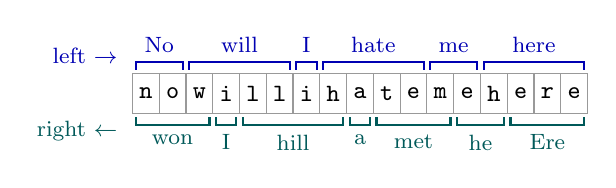
\begin{tikzpicture}[x=0.34cm, y=0.5cm, font=\small]
  \foreach \c [count=\i from 0] in {n,o,w,i,l,l,i,h,a,t,e,m,e,h,e,r,e} {
    \node[draw=black!40, minimum width=0.34cm, minimum height=0.5cm, inner sep=0pt, font=\ttfamily\small] at (\i,0) {\c};
  }
  % left words, read forward, above
  \foreach \a/\b/\t in {0/1/No, 2/5/will, 6/6/I, 7/10/hate, 11/12/me, 13/16/here} {
    \draw[blue!70!black, thick] (\a-0.38,0.6) -- (\a-0.38,0.8) -- (\b+0.38,0.8) -- (\b+0.38,0.6);
    \node[blue!70!black, above, font=\footnotesize] at ({(\a+\b)/2},0.8) {\t};
  }
  % right words, read backward, below
  \foreach \a/\b/\t in {0/2/won, 3/3/I, 4/7/hill, 8/8/a, 9/11/met, 12/13/he, 14/16/Ere} {
    \draw[teal!70!black, thick] (\a-0.38,-0.6) -- (\a-0.38,-0.8) -- (\b+0.38,-0.8) -- (\b+0.38,-0.6);
    \node[teal!70!black, below, font=\footnotesize] at ({(\a+\b)/2},-0.8) {\t};
  }
  \node[anchor=east, blue!70!black, font=\footnotesize] at (-0.7,0.95) {left $\rightarrow$};
  \node[anchor=east, teal!70!black, font=\footnotesize] at (-0.7,-0.95) {right $\leftarrow$};
\end{tikzpicture}

\vspace{4pt}
\footnotesize
\setlength{\tabcolsep}{4pt}
\begin{tabular}{@{}r l l l l@{}}
\toprule
& Side & Word & Effect & Next debt \\
\midrule
1 & L & here & opens shell & R owes \code{ereh} \\
2 & R & Ere & pays & R owes \code{h} \\
3 & R & he & overpays & L owes \code{e} \\
4 & L & me & overpays & R owes \code{m} \\
5 & R & met & overpays & L owes \code{te} \\
6 & L & hate & overpays & R owes \code{ah} \\
7 & R & a & pays & R owes \code{h} \\
8 & R & hill & overpays & L owes \code{lli} \\
9 & L & I & pays & L owes \code{ll} \\
10 & L & will & overpays & R owes \code{iw} \\
11 & R & I & pays & R owes \code{w} \\
12 & R & won & overpays & L owes \code{no} \\
13 & L & No & pays & settled \\
\bottomrule
\end{tabular}
\caption{Debt crossing on \w{No, will I hate me here? / Ere he met a hill. I won.} Top: the shared letter string, segmented by the left half read forward (above) and by the right half read backward (below); boundaries align only at the ends. Bottom: the move sequence. Seven of the thirteen moves overpay and hand the reversed surplus to the other side. Full stops and commas are free moves and are omitted; the generator emits only commas and full stops, and the question mark is shown for the reader. The pair \w{I hate me here} $|$ \w{Ere he met a hill} occurs in deployed output.}
\label{fig:example}
\end{figure}

\subsection{Scoring}
\paragraph{Prose model.} A trigram model with stupid backoff \citep{brants-etal-2007-large} is trained on the Brown corpus and the NLTK Gutenberg selection (Austen, Melville, Carroll, Chesterton, the King James Bible, Milton, Whitman, Shakespeare; 3.8M tokens), lower-cased, with commas and full stops as tokens and the full stop doubling as the sentence boundary. Trigrams and bigrams seen fewer than twice are dropped. The whole paragraph is scored in one direction, forward. Appending on the right adds the terms of the new tokens. Prepending on the left adds the terms of the new tokens and re-scores the two tokens that follow them, whose context has changed; the leftmost token is scored on backoff until something is prepended. Every state's score is therefore the forward score of its current text, and states with different growth histories compare fairly. Candidate pruning for left moves uses the backward conditional $P(w \mid b\,c)$ from the same counts.

\paragraph{Sentence verifier.} When a full stop closes a sentence on either half, the verifier of \S\ref{sec:verifier} returns a readability probability $r$ for the closed sentence of $n$ words, and the state receives
\[
  2\,\bigl(\log\max(r, 0.02) - \log 0.5\bigr)\cdot \min(n,12)/4 .
\]
Fragments and word salad pay; real clauses earn in proportion to their length, up to twelve words.

\paragraph{Penalties.} Content words (three or more letters, not a function word) receive a bonus of 1.6 on use, minus 4 per earlier use within the last 40 tokens on that edge and 0.5 per use elsewhere; any word occurring twice within the nine tokens at the growing edge pays 4; function words pay 0.6 per use beyond three in the recent window. A word pair already present in the paragraph pays 6, which stops the cycles that a mirror invites. An edge with no full stop in its last 18 tokens pays 2 per new word (run-on). Each comma costs 1.

\paragraph{Theme.} Optional theme words select a topic vector. Each vocabulary word has a tf--idf vector over 2,000-word passages of the same corpora; a word's theme bonus is its cosine with the centroid of the theme words, kept for the 3,000 nearest words. The bonus (weight 15 in production) is paid on a word's first use only; afterwards the word is ordinary repetition.

\subsection{Beam, diversity and closure}
States are ranked by priority $\text{score} + 0.7\,|\lambda(s)| - 0.4\,|d|$, which rewards letters placed and charges unpaid debt. Each parent contributes its 12 best children. To prevent the beam from filling with near-copies, states are merged on the key (first three tokens, last three tokens, owing side, debt) and the best of each key survives; a uniform random term in $[0, 4)$ is added to priorities for the first eight steps, then in $[0, 0.3)$. A settled state with at least the target number of letters, not starting with punctuation and not ending in a comma, is closed: its first and last tokens are re-scored against sentence boundaries and its outermost sentences are judged by the verifier. Closed paragraphs are ranked by score per token. States more than a slack of letters beyond the target are dropped, so the search terminates. Production settings are 300 target letters, beam 200 and slack 40 (Appendix~\ref{app:settings}).

Exactness holds by construction: every move preserves the debt invariant, and closure requires zero debt. We also check it independently on every output (\S\ref{sec:results}).

\section{A count-based readability verifier}\label{sec:verifier}

The verifier scores a sentence from counts in about \verifierMs{}~ms (warm, single thread, measured on the \vFiveLiveN{} deployed paragraphs' sentences), cheap enough to call on every closed sentence in the beam.

\paragraph{Syntax gain.} Words are tagged by a Viterbi-style search over Brown tags (normalised, 12 best histories). Each word's candidate tags are those covering at least 2\% of its Brown occurrences; unknown words get suffix-based guesses, and a capitalised word inside a clause may be a proper noun. Tag transitions interpolate trigram, bigram and unigram estimates (0.6/0.3/0.1). For the best path, each step's \emph{gain} is $\log P(\text{tag}_i \mid \text{tag}_{i-2}\,\text{tag}_{i-1}) - \log P(\text{tag}_i)$, including the end-of-clause step. Word salad takes steps Brown never takes and shows large negative gains.

\paragraph{Readable axis.} Three features enter a logistic model: mean gain, the mean of the two worst gains, and the filler share (function words and words of at most two letters). Positives are \anchorReddit{} human palindromes posted to an online forum, \anchorBrown{} short Brown sentences and the \anchorClassics{} classics; negatives are \anchorVOneWindows{} windows of four to eleven words from \anchorVOneOutputs{} long v1 outputs and the \anchorShuffled{} human palindromes with their words shuffled. Five-fold held-out AUC is \verifierAUC{}. Two fixed penalties follow the logistic: twice the repetition rate (repeated content words plus twice the repeated bigrams, per word) and 1.5 times the share of non-words above 15\%.

\paragraph{Spectrum.} A second axis, \emph{ism}, measures how stock a text is: mean web-bigram surprisal of its joins \citep{norvig-2009-ngrams} plus mean word rarity ($7.5-\text{Zipf}$), mapped linearly so that stock phrases sit at 1, raised to the text's overlap with a classic palindrome. Readable text at the garbage end is salad; at the stock end it is a retread. The verifier's combined score rewards readable text at ism 0.2, the region where human forum palindromes fall. v5's beam uses only the readable axis; we report ism as a measurement.

\section{Evaluation}\label{sec:eval}

\paragraph{Corpora.} \textbf{v5 live}: \vFiveLiveN{} paragraphs from the deployed generator (production settings, random seeds, no theme unless the user prompt supplies one; collected before the theme draw of Table~\ref{tab:themes}), \vFiveLiveLettersMin--\vFiveLiveLettersMax{} letters. \textbf{v5 long}: \vFiveSophiaN{} themed paragraphs of \vFiveSophiaLettersMin--\vFiveSophiaLettersMax{} letters from \longBatches{} development batches on a CPU cluster (\longThemes{} three-word themes such as \w{sea, ship, storm}; targets \longTargetMin--\longTargetMax{} letters; beams \longBeamMin--\longBeamMax; \longSecsMin--\longSecsMax{}\,s per paragraph, median \longSecsMed{}\,s). The generator code changed between batches, so this corpus represents the v5 family at length, not a controlled ablation. \textbf{v1}: \vOneN{} fresh outputs of the archived v1 code run in archive mode with its GPT-2 reranker loaded (\nolinkurl{data/spectrum-anchors/v1-archive-50-20261125.jsonl}); the search returns the same few texts across runs, so the \vOneN{} outputs contain only \vOneDistinct{} distinct texts and v1's per-paragraph statistics carry little more information than \vOneDistinct{} samples. The live v5 corpus contains \vFiveLiveDistinct{} distinct texts and the long corpus \vFiveSophiaDistinct. \textbf{Brown}: \BrownN{} contiguous passages of about 100 words from the Brown corpus (fixed seed). \textbf{Classics}: the \ClassicsN{} famous human palindromes the verifier uses as anchors (\w{a man a plan a canal panama}), \ClassicsLettersMin--\ClassicsLettersMax{} letters.

\paragraph{Metrics.} \emph{Exactness}: letters only, compared with their reverse. \emph{Short-word share}: words of one or two letters. \emph{Type--token ratio} and \emph{distinct bigrams} (unique word bigrams over all bigrams). \emph{Words per sentence}, splitting on \code{.!?}. \emph{Trigram LM}: mean stupid-backoff log score per token, boundaries included, under v5's own prose model. \emph{Verifier}: each sentence of at least two words is scored; we report the mean readability probability, the share of sentences at or above 0.6 (\emph{readable}) and below 0.3 (\emph{garbage}), averaged over paragraphs, and mean ism. \emph{GPT-2 perplexity}: the 124M-parameter model on the rendered text with its capitals and punctuation, first 1,024 tokens, median over paragraphs. Classics are excluded from perplexity: at a median of \ClassicsLettersMed{} letters, a few tokens dominate it.

\paragraph{Independence.} The trigram LM and the verifier are terms of v5's objective; rows that use them are marked \obj{} and are reported as a check that the search does what it is built to do. GPT-2 never enters the search, the lexicon or the tuning, so it is the one independent automatic signal. It is not a reader.

\section{Results}\label{sec:results}

\begin{table}[t]
\centering\footnotesize
\setlength{\tabcolsep}{2.6pt}
\begin{tabular}{@{}l r r r r r@{}}
\toprule
& v1 & \multicolumn{2}{c}{v5} & Brown & Class. \\
\cmidrule(lr){3-4}
& & live & long & & \\
\midrule
$n$ & \vOneN & \vFiveLiveN & \vFiveSophiaN & \BrownN & \ClassicsN \\
Letters (mean) & \vOneLetters & \vFiveLiveLetters & \vFiveSophiaLetters & \BrownLetters & \ClassicsLetters \\
Exact (\%) & \vOneExact & \vFiveLiveExact & \vFiveSophiaExact & \BrownExact & \ClassicsExact \\
Short words (\%) & \vOneShort & \vFiveLiveShort & \vFiveSophiaShort & \BrownShort & \ClassicsShort \\
Word length & \vOneWordLen & \vFiveLiveWordLen & \vFiveSophiaWordLen & \BrownWordLen & \ClassicsWordLen \\
Type--token & \vOneTTR & \vFiveLiveTTR & \vFiveSophiaTTR & \BrownTTR & \ClassicsTTR \\
Distinct bigr. (\%) & \vOneBigrams & \vFiveLiveBigrams & \vFiveSophiaBigrams & \BrownBigrams & \ClassicsBigrams \\
Words/sentence & \vOneSentWords & \vFiveLiveSentWords & \vFiveSophiaSentWords & \BrownSentWords & \ClassicsSentWords \\
\midrule
Trigram LM\obj & \vOneLM & \vFiveLiveLM & \vFiveSophiaLM & \BrownLM & \ClassicsLM \\
Readable mean\obj & \vOneReadable & \vFiveLiveReadable & \vFiveSophiaReadable & \BrownReadable & \ClassicsReadable \\
Readable (\%)\obj & \vOneReadableShare & \vFiveLiveReadableShare & \vFiveSophiaReadableShare & \BrownReadableShare & \ClassicsReadableShare \\
Garbage (\%)\obj & \vOneGarbageShare & \vFiveLiveGarbageShare & \vFiveSophiaGarbageShare & \BrownGarbageShare & \ClassicsGarbageShare \\
Ism & \vOneIsm & \vFiveLiveIsm & \vFiveSophiaIsm & \BrownIsm & \ClassicsIsm \\
\midrule
GPT-2 ppl & \vOnePPL & \vFiveLivePPL & \vFiveSophiaPPL & \BrownPPL & -- \\
\quad IQR & {\scriptsize\vOnePPLQone--\vOnePPLQthree} & {\scriptsize\vFiveLivePPLQone--\vFiveLivePPLQthree} & {\scriptsize\vFiveSophiaPPLQone--\vFiveSophiaPPLQthree} & {\scriptsize\BrownPPLQone--\BrownPPLQthree} & -- \\
\bottomrule
\end{tabular}
\caption{Per-corpus means; GPT-2 perplexity is the median with its interquartile range. Readable and garbage are shares of sentences. \obj{}Term of v5's search objective: not independent evidence. GPT-2 never enters the search.}
\label{tab:main}
\end{table}

\paragraph{Exactness.} Every generated paragraph is exact: \vFiveLiveExactCheck/\vFiveLiveN{} live, \vFiveSophiaExactCheck/\vFiveSophiaN{} long, by an independent letters-only check as well as the project's validator. The long corpus reaches \vFiveSophiaLettersMax{} letters.

\paragraph{The objective is met, which proves little.} v5's sentences score \vFiveLiveReadable{} on the verifier against \BrownReadable{} for Brown, with \vFiveLiveReadableShare\% of sentences readable against \BrownReadableShare\% (Table~\ref{tab:main}, Figure~\ref{fig:dist}c). Under its own trigram model, v5 text scores \vFiveLiveLM{} per token, \emph{higher} than Brown's \BrownLM. Neither comparison says v5 reads as well as Brown. The search was built to maximise both quantities, and it does. They show that the objective is implemented correctly and that it is saturated: further optimisation against these scores cannot be measured by them. The verifier does separate v1 (\vOneReadable{} readable mean, \vOneGarbageShare\% of sentences garbage) from everything else, which is the distinction it was fitted to make.

\begin{figure}[t]
\centering
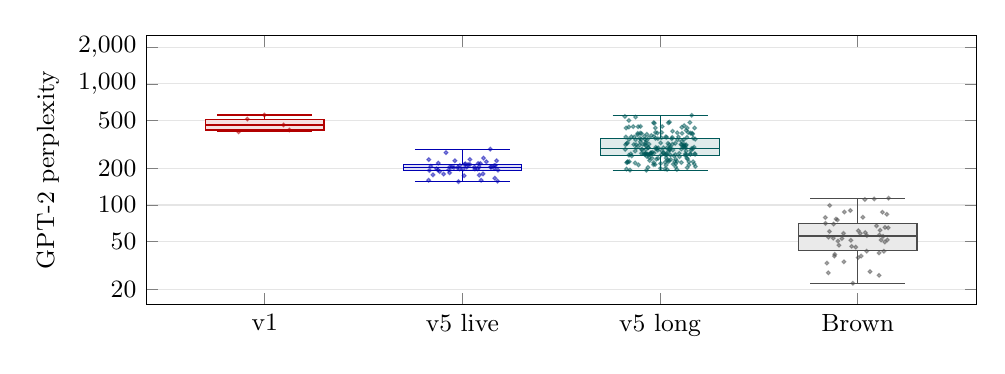
\begin{tikzpicture}
\begin{axis}[
  width=\columnwidth, height=5.0cm,
  ymode=log, log basis y=10, ytick={20,50,100,200,500,1000,2000}, log ticks with fixed point,
  ylabel={GPT-2 perplexity}, ylabel style={font=\small},
  xtick={1,2,3,4}, xticklabels={v1, v5 live, v5 long, Brown},
  tick label style={font=\small},
  xmin=0.4, xmax=4.6, ymin=15, ymax=2500,
  ymajorgrids, grid style={black!10},
  boxplot/draw direction=y,
]
% v1: n=5
\addplot+[boxplot prepared={draw position=1, lower whisker=401.3, lower quartile=415.4, median=457.3, upper quartile=511.2, upper whisker=552.5, box extend=0.6}, draw=cvOne, solid, fill=cvOne!12, mark=none] coordinates {};
\addplot[only marks, mark=*, mark size=0.7pt, cvOne, opacity=0.45] coordinates {(0.868,401.3) (1.125,415.4) (1.095,457.3) (0.912,511.2) (0.998,552.5)};
% v5_live: n=50
\addplot+[boxplot prepared={draw position=2, lower whisker=155.9, lower quartile=193, median=205.3, upper quartile=216.4, upper whisker=288.7, box extend=0.6}, draw=cLive, solid, fill=cLive!12, mark=none] coordinates {};
\addplot[only marks, mark=*, mark size=0.7pt, cLive, opacity=0.45] coordinates {(2.164,166.4) (2.161,211) (1.840,208.8) (1.851,177.2) (2.121,227.4) (2.085,176.4) (2.061,205.3) (1.931,194.5) (2.038,237.7) (2.038,215.8) (2.029,215.8) (1.877,194.1) (1.975,203.6) (1.962,231.4) (2.080,220.1) (2.178,157.3) (2.162,200.1) (2.016,218.3) (1.980,155.9) (1.917,270.5) (1.833,192.7) (1.830,236.9) (1.987,211.5) (1.935,184.4) (1.957,203.6) (2.141,288.7) (2.009,174.1) (2.022,205.3) (1.905,179.8) (1.829,160) (1.937,206.2) (1.869,199.1) (2.004,198.2) (2.180,194.1) (2.063,198.2) (1.885,188.6) (2.142,205.3) (2.107,243.6) (2.084,205.3) (2.146,205.3) (2.095,160) (2.104,180.5) (1.947,205.8) (2.173,231.4) (2.166,211.3) (1.878,221.5) (2.091,219.7) (2.077,198.2) (1.986,198.2) (2.011,216.5)};
% v5_sophia: n=198
\addplot+[boxplot prepared={draw position=3, lower whisker=193.3, lower quartile=256.7, median=294.3, upper quartile=355.7, upper whisker=549.3, box extend=0.6}, draw=cLong, solid, fill=cLong!12, mark=none] coordinates {};
\addplot[only marks, mark=*, mark size=0.7pt, cLong, opacity=0.45] coordinates {(2.906,266.3) (3.016,268.8) (2.953,264.3) (3.037,234.7) (3.045,233.2) (2.844,228) (2.825,314) (3.121,316) (2.913,316.3) (2.904,349) (3.178,349) (2.989,352.8) (3.121,302.3) (2.991,295.6) (3.050,296.3) (2.874,278.7) (3.049,287.7) (3.132,278.9) (3.008,396.9) (3.087,394.2) (3.062,361.3) (2.843,348.3) (3.093,364) (3.033,362.2) (2.928,307.5) (2.831,320.9) (3.132,314.5) (2.990,243) (3.079,238.2) (3.136,243.3) (3.077,261.1) (3.152,262.9) (2.962,272.1) (3.108,289.5) (2.980,290) (3.157,281.8) (3.136,362) (2.855,365.4) (2.869,363.6) (2.898,355.4) (3.168,355.8) (2.977,354.5) (3.046,313.9) (2.928,328) (3.003,325.1) (2.959,243.4) (2.946,245) (3.031,244) (3.030,213.3) (3.146,214) (3.066,217.2) (3.154,262.4) (3.128,263.2) (3.177,261.9) (3.062,317.1) (2.879,314.5) (3.130,309) (3.167,227.1) (3.146,226.7) (3.025,225.3) (3.077,322.3) (2.896,311.6) (3.119,309.1) (3.026,260.1) (2.923,260.8) (2.843,257.9) (3.127,256.3) (3.176,265.2) (2.852,263.7) (3.108,224) (2.968,223.8) (2.874,222.2) (2.926,266.4) (3.097,267.2) (3.134,258.3) (2.836,227.1) (3.041,226.7) (2.836,225.3) (3.079,205.9) (2.939,204.2) (3.137,203.1) (3.173,217.8) (3.002,200.3) (3.179,207.5) (2.931,193.3) (2.848,194) (3.036,196.3) (2.831,223.6) (2.891,214) (2.967,215.3) (3.040,322.9) (2.876,345.5) (2.835,325.6) (3.132,412.4) (2.933,383.2) (3.165,385.1) (3.143,396) (2.956,374.3) (2.986,392.3) (3.007,259.7) (3.052,258.3) (3.034,295.1) (3.021,268.3) (3.043,275.8) (3.159,291.3) (3.003,219.9) (2.975,215.3) (3.079,218.7) (2.906,287.5) (2.928,286.8) (3.172,299.9) (3.008,279.6) (3.017,296.4) (2.824,287.6) (2.969,367.9) (3.029,364.5) (2.827,363.6) (3.042,477.1) (3.048,483) (2.842,498.1) (3.046,284.6) (2.988,283.4) (3.065,284.1) (2.947,232.4) (3.075,228.8) (3.086,229.1) (2.828,431.6) (2.842,439.8) (3.063,405.9) (3.167,293.5) (2.910,286.2) (2.984,292.9) (3.033,263.2) (2.935,262.8) (2.951,263.1) (2.933,250.9) (2.953,269.1) (3.034,258.4) (2.928,264) (2.956,268.9) (3.098,250.3) (2.830,197.8) (3.025,198.7) (3.085,196.3) (2.932,339.6) (2.900,332.4) (3.109,335.2) (2.906,388.7) (2.887,389.9) (2.977,397) (3.071,253) (2.857,254.3) (2.936,261) (2.940,296.5) (3.120,299.8) (2.978,298.8) (3.128,297) (2.881,297.3) (2.941,298.4) (3.054,236.8) (3.139,239.3) (2.982,238.6) (2.901,444.6) (2.864,443.4) (3.011,444.2) (2.889,442.5) (3.110,437.2) (3.122,451.5) (2.886,379.2) (2.920,368.1) (3.111,390.5) (3.051,301.3) (3.110,313.1) (2.944,318) (2.867,315.7) (2.925,315.9) (3.106,316) (2.918,265.5) (2.945,261.6) (2.970,268.1) (2.971,472.9) (2.967,477.6) (3.151,479.5) (2.876,531.7) (2.822,537.7) (3.160,549.3) (3.137,431.2) (3.175,431.9) (2.976,432.5) (3.162,390.3) (3.154,391.4) (2.900,391.9) (3.088,344.7) (3.121,347.1) (3.059,352.5) (3.007,358.7) (2.924,348.8) (2.943,358.1)};
% brown: n=50
\addplot+[boxplot prepared={draw position=4, lower whisker=22.57, lower quartile=42.38, median=55.47, upper quartile=70.22, upper whisker=113.7, box extend=0.6}, draw=cBrown, solid, fill=cBrown!12, mark=none] coordinates {};
\addplot[only marks, mark=*, mark size=0.7pt, cBrown, opacity=0.45] coordinates {(3.905,46.5) (3.857,60.39) (3.963,89.99) (3.876,53.16) (3.844,33.1) (3.965,51.09) (4.150,51.49) (4.108,26.25) (4.095,67.27) (3.900,50.38) (4.013,58.18) (3.920,52.76) (3.882,37.84) (3.858,99.05) (3.897,75.26) (4.154,64.72) (4.118,51.34) (4.110,56.53) (4.108,40.18) (3.890,76.56) (3.932,87.44) (4.046,55.93) (4.083,112.2) (4.128,55.01) (4.137,49.49) (3.851,27.53) (4.038,59.17) (4.062,28.19) (4.002,36.74) (3.884,39.16) (3.990,44.83) (3.852,54.22) (4.156,113.7) (4.132,41.51) (4.017,37.87) (3.928,58.17) (4.147,83.81) (4.026,79.22) (4.138,65.33) (4.125,87.09) (4.003,61.36) (3.969,45.49) (4.036,110.9) (3.975,22.57) (3.878,69.58) (3.930,33.92) (4.113,61.95) (3.836,78.76) (3.837,70.43) (4.045,41.56)};

\end{axis}
\end{tikzpicture}
\caption{GPT-2 perplexity per paragraph (log scale). Boxes span the interquartile range with the median; whiskers reach the extremes; points are paragraphs. GPT-2 is outside the search. \inBrownRangeLive{} live and \inBrownRangeLong{} long paragraphs reach Brown's range; \belowVOneMinLive{} of \vFiveLiveN{} live paragraphs fall below v1's minimum.}
\label{fig:ppl}
\end{figure}

\paragraph{Independent check: GPT-2.} GPT-2's median perplexity on v5 live is \vFiveLivePPL{} against \vOnePPL{} for v1, a factor of \pplRatioVOne{} (Figure~\ref{fig:ppl}). All \belowVOneMinLive{} of \vFiveLiveN{} live paragraphs fall below the lowest v1 value, and \belowVOneMinLong{} of \vFiveSophiaN{} long ones do. Brown's median is \BrownPPL: v5 live is \pplRatioBrownLive{} times higher, the long corpus \pplRatioBrownLong{} times. The two distributions do not overlap: \inBrownRangeLive{} live and \inBrownRangeLong{} long paragraphs fall at or below Brown's maximum of \BrownPPLMax. Part of the gain over v1 comes from vocabulary, since v1 admits web tokens such as \w{hdr} and \w{nintendo}, and part from presentation: v1 outputs are one unpunctuated lower-case run (\vOneSentWords{} words per sentence), while v5 emits capitals and full stops every \vFiveLiveSentWords{} words, and GPT-2 rewards both. Sentence boundaries are a search decision in v5 and part of its contribution, but a control that renders v5 without punctuation is needed to size that share.

\begin{figure*}[t]
\centering
\pgfplotsset{distpanel/.style={
  width=0.36\textwidth, height=4.4cm,
  title style={font=\small, yshift=-4pt},
  xtick={1,2,3,4,5}, xticklabels={v1, v5 live, v5 long, Brown, Classics},
  x tick label style={font=\scriptsize, rotate=30, anchor=north east, inner sep=1pt},
  y tick label style={font=\scriptsize},
  xmin=0.4, xmax=5.6, ymajorgrids, grid style={black!10}, boxplot/draw direction=y}}
\begin{tikzpicture}
\begin{axis}[distpanel, name=a, title={(a) Letters per paragraph}, ymin=0, ymax=1100]
% v1: n=5
\addplot+[boxplot prepared={draw position=1, lower whisker=354.0000, lower quartile=474.0000, median=478.0000, upper quartile=514.0000, upper whisker=516.0000, box extend=0.6}, draw=cvOne, solid, fill=cvOne!12, mark=none] coordinates {};
\addplot[only marks, mark=*, mark size=0.7pt, cvOne, opacity=0.45] coordinates {(0.868,478.0000) (1.125,354.0000) (1.095,514.0000) (0.912,474.0000) (0.998,516.0000)};
% v5_live: n=50
\addplot+[boxplot prepared={draw position=2, lower whisker=300.0000, lower quartile=308.0000, median=321.0000, upper quartile=334.0000, upper whisker=340.0000, box extend=0.6}, draw=cLive, solid, fill=cLive!12, mark=none] coordinates {};
\addplot[only marks, mark=*, mark size=0.7pt, cLive, opacity=0.45] coordinates {(2.164,304.0000) (2.161,340.0000) (1.840,308.0000) (1.851,300.0000) (2.121,302.0000) (2.085,304.0000) (2.061,314.0000) (1.931,340.0000) (2.038,308.0000) (2.038,308.0000) (2.029,308.0000) (1.877,302.0000) (1.975,326.0000) (1.962,328.0000) (2.080,306.0000) (2.178,322.0000) (2.162,338.0000) (2.016,330.0000) (1.980,302.0000) (1.917,300.0000) (1.833,332.0000) (1.830,320.0000) (1.987,306.0000) (1.935,332.0000) (1.957,326.0000) (2.141,302.0000) (2.009,322.0000) (2.022,334.0000) (1.905,334.0000) (1.829,312.0000) (1.937,308.0000) (1.869,326.0000) (2.004,334.0000) (2.180,302.0000) (2.063,334.0000) (1.885,338.0000) (2.142,314.0000) (2.107,310.0000) (2.084,334.0000) (2.146,334.0000) (2.095,312.0000) (2.104,302.0000) (1.947,340.0000) (2.173,328.0000) (2.166,314.0000) (1.878,338.0000) (2.091,314.0000) (2.077,334.0000) (1.986,334.0000) (2.011,334.0000)};
% v5_sophia: n=198
\addplot+[boxplot prepared={draw position=3, lower whisker=600.0000, lower quartile=671.0000, median=708.0000, upper quartile=1000.0000, upper whisker=1064.0000, box extend=0.6}, draw=cLong, solid, fill=cLong!12, mark=none] coordinates {};
\addplot[only marks, mark=*, mark size=0.7pt, cLong, opacity=0.45] coordinates {(2.906,704.0000) (3.016,706.0000) (2.953,728.0000) (3.037,702.0000) (3.045,702.0000) (2.844,706.0000) (2.825,714.0000) (3.121,714.0000) (2.913,714.0000) (2.904,704.0000) (3.178,702.0000) (2.989,702.0000) (3.121,722.0000) (2.991,722.0000) (3.050,722.0000) (2.874,740.0000) (3.049,722.0000) (3.132,740.0000) (3.008,702.0000) (3.087,714.0000) (3.062,700.0000) (2.843,728.0000) (3.093,716.0000) (3.033,718.0000) (2.928,754.0000) (2.831,720.0000) (3.132,742.0000) (2.990,700.0000) (3.079,700.0000) (3.136,700.0000) (3.077,710.0000) (3.152,710.0000) (2.962,720.0000) (3.108,704.0000) (2.980,704.0000) (3.157,704.0000) (3.136,706.0000) (2.855,716.0000) (2.869,716.0000) (2.898,702.0000) (3.168,706.0000) (2.977,708.0000) (3.046,720.0000) (2.928,716.0000) (3.003,716.0000) (2.959,728.0000) (2.946,728.0000) (3.031,728.0000) (3.030,704.0000) (3.146,704.0000) (3.066,700.0000) (3.154,702.0000) (3.128,702.0000) (3.177,704.0000) (3.062,722.0000) (2.879,722.0000) (3.130,724.0000) (3.167,714.0000) (3.146,702.0000) (3.025,714.0000) (3.077,726.0000) (2.896,782.0000) (3.119,732.0000) (3.026,708.0000) (2.923,708.0000) (2.843,708.0000) (3.127,702.0000) (3.176,702.0000) (2.852,702.0000) (3.108,714.0000) (2.968,702.0000) (2.874,714.0000) (2.926,702.0000) (3.097,702.0000) (3.134,702.0000) (2.836,714.0000) (3.041,702.0000) (2.836,714.0000) (3.079,706.0000) (2.939,702.0000) (3.137,702.0000) (3.173,702.0000) (3.002,724.0000) (3.179,708.0000) (2.931,706.0000) (2.848,706.0000) (3.036,706.0000) (2.831,702.0000) (2.891,722.0000) (2.967,722.0000) (3.040,608.0000) (2.876,610.0000) (2.835,600.0000) (3.132,610.0000) (2.933,614.0000) (3.165,614.0000) (3.143,662.0000) (2.956,674.0000) (2.986,680.0000) (3.007,680.0000) (3.052,680.0000) (3.034,600.0000) (3.021,604.0000) (3.043,600.0000) (3.159,610.0000) (3.003,602.0000) (2.975,628.0000) (3.079,602.0000) (2.906,1054.0000) (2.928,1054.0000) (3.172,1008.0000) (3.008,1002.0000) (3.017,1000.0000) (2.824,1006.0000) (2.969,1010.0000) (3.029,1010.0000) (2.827,1010.0000) (3.042,1008.0000) (3.048,1008.0000) (2.842,1012.0000) (3.046,1020.0000) (2.988,1020.0000) (3.065,1020.0000) (2.947,1032.0000) (3.075,1014.0000) (3.086,1014.0000) (2.828,624.0000) (2.842,614.0000) (3.063,622.0000) (3.167,650.0000) (2.910,670.0000) (2.984,650.0000) (3.033,610.0000) (2.935,610.0000) (2.951,610.0000) (2.933,612.0000) (2.953,612.0000) (3.034,616.0000) (2.928,618.0000) (2.956,614.0000) (3.098,622.0000) (2.830,602.0000) (3.025,602.0000) (3.085,602.0000) (2.932,1012.0000) (2.900,1024.0000) (3.109,1000.0000) (2.906,1006.0000) (2.887,1018.0000) (2.977,1008.0000) (3.071,1042.0000) (2.857,1048.0000) (2.936,1064.0000) (2.940,1000.0000) (3.120,1000.0000) (2.978,1000.0000) (3.128,1000.0000) (2.881,1000.0000) (2.941,1028.0000) (3.054,1010.0000) (3.139,1004.0000) (2.982,1010.0000) (2.901,600.0000) (2.864,600.0000) (3.011,600.0000) (2.889,602.0000) (3.110,602.0000) (3.122,602.0000) (2.886,600.0000) (2.920,600.0000) (3.111,602.0000) (3.051,600.0000) (3.110,600.0000) (2.944,600.0000) (2.867,600.0000) (2.925,600.0000) (3.106,600.0000) (2.918,600.0000) (2.945,604.0000) (2.970,600.0000) (2.971,1002.0000) (2.967,1002.0000) (3.151,1002.0000) (2.876,1000.0000) (2.822,1000.0000) (3.160,1000.0000) (3.137,1000.0000) (3.175,1000.0000) (2.976,1000.0000) (3.162,1004.0000) (3.154,1004.0000) (2.900,1004.0000) (3.088,1000.0000) (3.121,1004.0000) (3.059,1000.0000) (3.007,1000.0000) (2.924,1004.0000) (2.943,1000.0000)};
% brown: n=50
\addplot+[boxplot prepared={draw position=4, lower whisker=296.0000, lower quartile=382.7500, median=459.0000, upper quartile=538.2500, upper whisker=624.0000, box extend=0.6}, draw=cBrown, solid, fill=cBrown!12, mark=none] coordinates {};
\addplot[only marks, mark=*, mark size=0.7pt, cBrown, opacity=0.45] coordinates {(3.905,448.0000) (3.857,595.0000) (3.963,353.0000) (3.876,589.0000) (3.844,371.0000) (3.965,439.0000) (4.150,516.0000) (4.108,472.0000) (4.095,527.0000) (3.900,441.0000) (4.013,319.0000) (3.920,459.0000) (3.882,624.0000) (3.858,478.0000) (3.897,367.0000) (4.154,560.0000) (4.118,485.0000) (4.110,561.0000) (4.108,461.0000) (3.890,444.0000) (3.932,396.0000) (4.046,487.0000) (4.083,414.0000) (4.128,387.0000) (4.137,385.0000) (3.851,471.0000) (4.038,382.0000) (4.062,364.0000) (4.002,296.0000) (3.884,589.0000) (3.990,571.0000) (3.852,355.0000) (4.156,351.0000) (4.132,490.0000) (4.017,332.0000) (3.928,346.0000) (4.147,610.0000) (4.026,588.0000) (4.138,571.0000) (4.125,464.0000) (4.003,525.0000) (3.969,566.0000) (4.036,459.0000) (3.975,365.0000) (3.878,445.0000) (3.930,451.0000) (4.113,388.0000) (3.836,542.0000) (3.837,616.0000) (4.045,351.0000)};
% classics: n=38
\addplot+[boxplot prepared={draw position=5, lower whisker=7.0000, lower quartile=11.0000, median=13.0000, upper quartile=18.5000, upper whisker=34.0000, box extend=0.6}, draw=cClassic, solid, fill=cClassic!12, mark=none] coordinates {};
\addplot[only marks, mark=*, mark size=0.7pt, cClassic, opacity=0.45] coordinates {(5.044,21.0000) (5.087,12.0000) (5.106,19.0000) (5.159,14.0000) (5.086,11.0000) (5.152,12.0000) (4.830,14.0000) (4.988,13.0000) (5.160,20.0000) (5.054,13.0000) (5.144,12.0000) (4.861,11.0000) (4.989,21.0000) (4.909,17.0000) (5.016,11.0000) (5.027,11.0000) (4.825,12.0000) (4.898,11.0000) (4.921,7.0000) (5.150,13.0000) (5.096,10.0000) (4.877,26.0000) (5.107,19.0000) (4.870,9.0000) (5.042,16.0000) (4.866,7.0000) (4.821,14.0000) (5.134,19.0000) (4.895,13.0000) (4.898,33.0000) (5.174,15.0000) (5.134,7.0000) (4.924,7.0000) (5.166,34.0000) (5.014,19.0000) (5.064,9.0000) (4.894,9.0000) (5.159,11.0000)};

\end{axis}
\begin{axis}[distpanel, name=b, at={(a.east)}, anchor=west, xshift=0.9cm, title={(b) Short-word share}, ymin=0, ymax=0.8]
% v1: n=5
\addplot+[boxplot prepared={draw position=1, lower whisker=0.4176, lower quartile=0.4199, median=0.4345, upper quartile=0.4419, upper whisker=0.4453, box extend=0.6}, draw=cvOne, solid, fill=cvOne!12, mark=none] coordinates {};
\addplot[only marks, mark=*, mark size=0.7pt, cvOne, opacity=0.45] coordinates {(0.868,0.4419) (1.125,0.4453) (1.095,0.4199) (0.912,0.4345) (0.998,0.4176)};
% v5_live: n=50
\addplot+[boxplot prepared={draw position=2, lower whisker=0.4159, lower quartile=0.4323, median=0.4483, upper quartile=0.4677, upper whisker=0.5207, box extend=0.6}, draw=cLive, solid, fill=cLive!12, mark=none] coordinates {};
\addplot[only marks, mark=*, mark size=0.7pt, cLive, opacity=0.45] coordinates {(2.164,0.4259) (2.161,0.4538) (1.840,0.4393) (1.851,0.4673) (2.121,0.4327) (2.085,0.4821) (2.061,0.4312) (1.931,0.4839) (2.038,0.4690) (2.038,0.4393) (2.029,0.4393) (1.877,0.4231) (1.975,0.4483) (1.962,0.4159) (2.080,0.4476) (2.178,0.5207) (2.162,0.4583) (2.016,0.4790) (1.980,0.4404) (1.917,0.4528) (1.833,0.4786) (1.830,0.4312) (1.987,0.4476) (1.935,0.4538) (1.957,0.4483) (2.141,0.4679) (2.009,0.5085) (2.022,0.4483) (1.905,0.4322) (1.829,0.4912) (1.937,0.4393) (1.869,0.5000) (2.004,0.4483) (2.180,0.4231) (2.063,0.4483) (1.885,0.4553) (2.142,0.4312) (2.107,0.4272) (2.084,0.4483) (2.146,0.4483) (2.095,0.4912) (2.104,0.4909) (1.947,0.5041) (2.173,0.4159) (2.166,0.4312) (1.878,0.4538) (2.091,0.4312) (2.077,0.4483) (1.986,0.4483) (2.011,0.4202)};
% v5_sophia: n=198
\addplot+[boxplot prepared={draw position=3, lower whisker=0.3115, lower quartile=0.3479, median=0.3797, upper quartile=0.4000, upper whisker=0.4350, box extend=0.6}, draw=cLong, solid, fill=cLong!12, mark=none] coordinates {};
\addplot[only marks, mark=*, mark size=0.7pt, cLong, opacity=0.45] coordinates {(2.906,0.4262) (3.016,0.4221) (2.953,0.4080) (3.037,0.4149) (3.045,0.4149) (2.844,0.4100) (2.825,0.3475) (3.121,0.3475) (2.913,0.3475) (2.904,0.3728) (3.178,0.3816) (2.989,0.3816) (3.121,0.3613) (2.991,0.3613) (3.050,0.3613) (2.874,0.3760) (3.049,0.3713) (3.132,0.3760) (3.008,0.3422) (3.087,0.3421) (3.062,0.3318) (2.843,0.3333) (3.093,0.3304) (3.033,0.3274) (2.928,0.3865) (2.831,0.3729) (3.132,0.3796) (2.990,0.4221) (3.079,0.4221) (3.136,0.4221) (3.077,0.3992) (3.152,0.3992) (2.962,0.4008) (3.108,0.3840) (2.980,0.3840) (3.157,0.3840) (3.136,0.3435) (2.855,0.3362) (2.869,0.3362) (2.898,0.3519) (3.168,0.3476) (2.977,0.3574) (3.046,0.3724) (2.928,0.3782) (3.003,0.3782) (2.959,0.3862) (2.946,0.3862) (3.031,0.3862) (3.030,0.4139) (3.146,0.4074) (3.066,0.4050) (3.154,0.4068) (3.128,0.4000) (3.177,0.4008) (3.062,0.3598) (2.879,0.3598) (3.130,0.3651) (3.167,0.3821) (3.146,0.3802) (3.025,0.3821) (3.077,0.3689) (2.896,0.3615) (3.119,0.3684) (3.026,0.3975) (2.923,0.3975) (2.843,0.3975) (3.127,0.3992) (3.176,0.3992) (2.852,0.3992) (3.108,0.3821) (2.968,0.3802) (2.874,0.3821) (2.926,0.4068) (3.097,0.4000) (3.134,0.3957) (2.836,0.3821) (3.041,0.3802) (2.836,0.3821) (3.079,0.4170) (2.939,0.4187) (3.137,0.4187) (3.173,0.4091) (3.002,0.4167) (3.179,0.4122) (2.931,0.4232) (2.848,0.4232) (3.036,0.4167) (2.831,0.3770) (2.891,0.3785) (2.967,0.3785) (3.040,0.3600) (2.876,0.3485) (2.835,0.3454) (3.132,0.3316) (2.933,0.3333) (3.165,0.3333) (3.143,0.3395) (2.956,0.3455) (2.986,0.3318) (3.007,0.3991) (3.052,0.3991) (3.034,0.3861) (3.021,0.3756) (3.043,0.3725) (3.159,0.3659) (3.003,0.4244) (2.975,0.4038) (3.079,0.4244) (2.906,0.3775) (2.928,0.3775) (3.172,0.3709) (3.008,0.3912) (3.017,0.3798) (2.824,0.3817) (2.969,0.3364) (3.029,0.3364) (2.827,0.3364) (3.042,0.3249) (3.048,0.3249) (2.842,0.3196) (3.046,0.3830) (2.988,0.3830) (3.065,0.3830) (2.947,0.4057) (3.075,0.4041) (3.086,0.4041) (2.828,0.3383) (2.842,0.3467) (3.063,0.3564) (3.167,0.3426) (2.910,0.3408) (2.984,0.3426) (3.033,0.3854) (2.935,0.3854) (2.951,0.3854) (2.933,0.4028) (2.953,0.4000) (3.034,0.4085) (2.928,0.4112) (2.956,0.4178) (3.098,0.4093) (2.830,0.4163) (3.025,0.4163) (3.085,0.4163) (2.932,0.3505) (2.900,0.3493) (3.109,0.3415) (2.906,0.3312) (2.887,0.3292) (2.977,0.3344) (3.071,0.3714) (2.857,0.3675) (2.936,0.3708) (2.940,0.3639) (3.120,0.3739) (2.978,0.3639) (3.128,0.3864) (2.881,0.3864) (2.941,0.3954) (3.054,0.4197) (3.139,0.4193) (2.982,0.4197) (2.901,0.3115) (2.864,0.3115) (3.011,0.3115) (2.889,0.3646) (3.110,0.3646) (3.122,0.3646) (2.886,0.3724) (2.920,0.3724) (3.111,0.3724) (3.051,0.3788) (3.110,0.3776) (2.944,0.3776) (2.867,0.4020) (2.925,0.4020) (3.106,0.4020) (2.918,0.4350) (2.945,0.4328) (2.970,0.4350) (2.971,0.3236) (2.967,0.3236) (3.151,0.3236) (2.876,0.3312) (2.822,0.3312) (3.160,0.3301) (3.137,0.3419) (3.175,0.3419) (2.976,0.3419) (3.162,0.3354) (3.154,0.3354) (2.900,0.3354) (3.088,0.3839) (3.121,0.3839) (3.059,0.3839) (3.007,0.3969) (2.924,0.3988) (2.943,0.3969)};
% brown: n=50
\addplot+[boxplot prepared={draw position=4, lower whisker=0.1000, lower quartile=0.1718, median=0.2025, upper quartile=0.2522, upper whisker=0.3299, box extend=0.6}, draw=cBrown, solid, fill=cBrown!12, mark=none] coordinates {};
\addplot[only marks, mark=*, mark size=0.7pt, cBrown, opacity=0.45] coordinates {(3.905,0.1333) (3.857,0.2049) (3.963,0.2000) (3.876,0.1700) (3.844,0.2644) (3.965,0.1584) (4.150,0.2286) (4.108,0.1236) (4.095,0.2362) (3.900,0.1717) (4.013,0.1750) (3.920,0.2128) (3.882,0.2883) (3.858,0.1000) (3.897,0.3152) (4.154,0.1827) (4.118,0.1556) (4.110,0.2097) (4.108,0.1786) (3.890,0.1739) (3.932,0.2903) (4.046,0.2083) (4.083,0.2000) (4.128,0.1209) (4.137,0.2381) (3.851,0.1566) (4.038,0.3125) (4.062,0.3299) (4.002,0.2533) (3.884,0.2500) (3.990,0.1786) (3.852,0.2588) (4.156,0.2674) (4.132,0.1982) (4.017,0.1282) (3.928,0.2558) (4.147,0.2328) (4.026,0.2056) (4.138,0.1776) (4.125,0.1531) (4.003,0.1261) (3.969,0.2544) (4.036,0.1720) (3.975,0.2209) (3.878,0.1944) (3.930,0.2200) (4.113,0.2824) (3.836,0.1667) (3.837,0.1780) (4.045,0.2529)};
% classics: n=38
\addplot+[boxplot prepared={draw position=5, lower whisker=0.0000, lower quartile=0.2292, median=0.3333, upper quartile=0.5000, upper whisker=0.7500, box extend=0.6}, draw=cClassic, solid, fill=cClassic!12, mark=none] coordinates {};
\addplot[only marks, mark=*, mark size=0.7pt, cClassic, opacity=0.45] coordinates {(5.044,0.4286) (5.087,0.5000) (5.106,0.5556) (5.159,0.2500) (5.086,0.3333) (5.152,0.2500) (4.830,0.5000) (4.988,0.2500) (5.160,0.3333) (5.054,0.2500) (5.144,0.5000) (4.861,0.3333) (4.989,0.2857) (4.909,0.4286) (5.016,0.3333) (5.027,0.3333) (4.825,0.0000) (4.898,0.3333) (4.921,0.0000) (5.150,0.0000) (5.096,0.7500) (4.877,0.5000) (5.107,0.2857) (4.870,0.0000) (5.042,0.0000) (4.866,0.0000) (4.821,0.5000) (5.134,0.3333) (4.895,0.6000) (4.898,0.2222) (5.174,0.6667) (5.134,0.3333) (4.924,0.6667) (5.166,0.1250) (5.014,0.3333) (5.064,0.5000) (4.894,0.0000) (5.159,0.0000)};

\end{axis}
\begin{axis}[distpanel, at={(b.east)}, anchor=west, xshift=0.9cm, title={(c) Readable sentences\obj}, ymin=-0.05, ymax=1.05]
% v1: n=5
\addplot+[boxplot prepared={draw position=1, lower whisker=0.0000, lower quartile=0.0000, median=0.0000, upper quartile=0.0000, upper whisker=0.0000, box extend=0.6}, draw=cvOne, solid, fill=cvOne!12, mark=none] coordinates {};
\addplot[only marks, mark=*, mark size=0.7pt, cvOne, opacity=0.45] coordinates {(0.868,0.0000) (1.125,0.0000) (1.095,0.0000) (0.912,0.0000) (0.998,0.0000)};
% v5_live: n=50
\addplot+[boxplot prepared={draw position=2, lower whisker=0.5000, lower quartile=0.6154, median=0.6667, upper quartile=0.7240, upper whisker=0.8125, box extend=0.6}, draw=cLive, solid, fill=cLive!12, mark=none] coordinates {};
\addplot[only marks, mark=*, mark size=0.7pt, cLive, opacity=0.45] coordinates {(2.164,0.7857) (2.161,0.8000) (1.840,0.7692) (1.851,0.7333) (2.121,0.6364) (2.085,0.5385) (2.061,0.6667) (1.931,0.6429) (2.038,0.6000) (2.038,0.6923) (2.029,0.6923) (1.877,0.7273) (1.975,0.8000) (1.962,0.7143) (2.080,0.7500) (2.178,0.6923) (2.162,0.6667) (2.016,0.5385) (1.980,0.7500) (1.917,0.5556) (1.833,0.6667) (1.830,0.6000) (1.987,0.7500) (1.935,0.7368) (1.957,0.8000) (2.141,0.5000) (2.009,0.5385) (2.022,0.6154) (1.905,0.6471) (1.829,0.6429) (1.937,0.6923) (1.869,0.6667) (2.004,0.6154) (2.180,0.7273) (2.063,0.6154) (1.885,0.6429) (2.142,0.6667) (2.107,0.6154) (2.084,0.6154) (2.146,0.6154) (2.095,0.6429) (2.104,0.7000) (1.947,0.6154) (2.173,0.7143) (2.166,0.6667) (1.878,0.8125) (2.091,0.6667) (2.077,0.6154) (1.986,0.6154) (2.011,0.5000)};
% v5_sophia: n=198
\addplot+[boxplot prepared={draw position=3, lower whisker=0.4000, lower quartile=0.5893, median=0.6500, upper quartile=0.7143, upper whisker=0.8462, box extend=0.6}, draw=cLong, solid, fill=cLong!12, mark=none] coordinates {};
\addplot[only marks, mark=*, mark size=0.7pt, cLong, opacity=0.45] coordinates {(2.906,0.6875) (3.016,0.6875) (2.953,0.6471) (3.037,0.6667) (3.045,0.6667) (2.844,0.7097) (2.825,0.5000) (3.121,0.4762) (2.913,0.4545) (2.904,0.7083) (3.178,0.6667) (2.989,0.6667) (3.121,0.6333) (2.991,0.6552) (3.050,0.6207) (2.874,0.6129) (3.049,0.6897) (3.132,0.6452) (3.008,0.6000) (3.087,0.6190) (3.062,0.5789) (2.843,0.6154) (3.093,0.6800) (3.033,0.6400) (2.928,0.6000) (2.831,0.6207) (3.132,0.5667) (2.990,0.7273) (3.079,0.7500) (3.136,0.7500) (3.077,0.5769) (3.152,0.5769) (2.962,0.5926) (3.108,0.7143) (2.980,0.7407) (3.157,0.7778) (3.136,0.6667) (2.855,0.7037) (2.869,0.7037) (2.898,0.5000) (3.168,0.5217) (2.977,0.5000) (3.046,0.6667) (2.928,0.6667) (3.003,0.6667) (2.959,0.6562) (2.946,0.6250) (3.031,0.6250) (3.030,0.7429) (3.146,0.7429) (3.066,0.7429) (3.154,0.6786) (3.128,0.7143) (3.177,0.6538) (3.062,0.7667) (2.879,0.7667) (3.130,0.7742) (3.167,0.7576) (3.146,0.7879) (3.025,0.7273) (3.077,0.6897) (2.896,0.6364) (3.119,0.7000) (3.026,0.7143) (2.923,0.7143) (2.843,0.7143) (3.127,0.7879) (3.176,0.7879) (2.852,0.7879) (3.108,0.7576) (2.968,0.7879) (2.874,0.7273) (2.926,0.6786) (3.097,0.7143) (3.134,0.7037) (2.836,0.7576) (3.041,0.7879) (2.836,0.7273) (3.079,0.7188) (2.939,0.6875) (3.137,0.6875) (3.173,0.7500) (3.002,0.7742) (3.179,0.7333) (2.931,0.7188) (2.848,0.7188) (3.036,0.7667) (2.831,0.6400) (2.891,0.6538) (2.967,0.6538) (3.040,0.6842) (2.876,0.6000) (2.835,0.6842) (3.132,0.5217) (2.933,0.5455) (3.165,0.5455) (3.143,0.4000) (2.956,0.4500) (2.986,0.4500) (3.007,0.7692) (3.052,0.7308) (3.034,0.7391) (3.021,0.7083) (3.043,0.6818) (3.159,0.6800) (3.003,0.7778) (2.975,0.7778) (3.079,0.8148) (2.906,0.6111) (2.928,0.6111) (3.172,0.6000) (3.008,0.5938) (3.017,0.5806) (2.824,0.6061) (2.969,0.5161) (3.029,0.5161) (2.827,0.5161) (3.042,0.4667) (3.048,0.4667) (2.842,0.4483) (3.046,0.6111) (2.988,0.6111) (3.065,0.6111) (2.947,0.6829) (3.075,0.6750) (3.086,0.6750) (2.828,0.6364) (2.842,0.6818) (3.063,0.6000) (3.167,0.6154) (2.910,0.6296) (2.984,0.5769) (3.033,0.6667) (2.935,0.6667) (2.951,0.6667) (2.933,0.5652) (2.953,0.5652) (3.034,0.5652) (2.928,0.7857) (2.956,0.7407) (3.098,0.7778) (2.830,0.8077) (3.025,0.8462) (3.085,0.8462) (2.932,0.5588) (2.900,0.6000) (3.109,0.5882) (2.906,0.6389) (2.887,0.6389) (2.977,0.6111) (3.071,0.6154) (2.857,0.6500) (2.936,0.6500) (2.940,0.5556) (3.120,0.5405) (2.978,0.5556) (3.128,0.6316) (2.881,0.6316) (2.941,0.6250) (3.054,0.7143) (3.139,0.6905) (2.982,0.7143) (2.901,0.5217) (2.864,0.5652) (3.011,0.5455) (2.889,0.4375) (3.110,0.4375) (3.122,0.4375) (2.886,0.5238) (2.920,0.5238) (3.111,0.5238) (3.051,0.7143) (3.110,0.7143) (2.944,0.7143) (2.867,0.6667) (2.925,0.6500) (3.106,0.6190) (2.918,0.5714) (2.945,0.5714) (2.970,0.5714) (2.971,0.5938) (2.967,0.5938) (3.151,0.5938) (2.876,0.5455) (2.822,0.5217) (3.160,0.5455) (3.137,0.5758) (3.175,0.5758) (2.976,0.5758) (3.162,0.6970) (3.154,0.6970) (2.900,0.6970) (3.088,0.6207) (3.121,0.6207) (3.059,0.6207) (3.007,0.6296) (2.924,0.6296) (2.943,0.6296)};
% brown: n=50
\addplot+[boxplot prepared={draw position=4, lower whisker=0.0000, lower quartile=0.5000, median=0.7500, upper quartile=0.8750, upper whisker=1.0000, box extend=0.6}, draw=cBrown, solid, fill=cBrown!12, mark=none] coordinates {};
\addplot[only marks, mark=*, mark size=0.7pt, cBrown, opacity=0.45] coordinates {(3.905,0.8000) (3.857,0.7500) (3.963,0.8182) (3.876,0.2500) (3.844,0.5000) (3.965,0.5714) (4.150,0.2000) (4.108,0.7143) (4.095,1.0000) (3.900,1.0000) (4.013,0.8571) (3.920,1.0000) (3.882,0.4000) (3.858,0.6000) (3.897,1.0000) (4.154,1.0000) (4.118,0.0000) (4.110,0.5000) (4.108,1.0000) (3.890,0.4000) (3.932,0.8750) (4.046,0.3333) (4.083,0.7500) (4.128,0.5000) (4.137,0.6667) (3.851,0.6667) (4.038,0.5714) (4.062,1.0000) (4.002,0.9167) (3.884,0.2000) (3.990,0.5000) (3.852,0.8000) (4.156,0.8750) (4.132,1.0000) (4.017,0.8750) (3.928,0.7778) (4.147,0.6000) (4.026,0.7500) (4.138,0.6000) (4.125,0.3333) (4.003,0.4000) (3.969,0.7500) (4.036,0.8000) (3.975,1.0000) (3.878,0.8571) (3.930,0.7143) (4.113,1.0000) (3.836,0.4000) (3.837,0.2500) (4.045,0.8750)};
% classics: n=38
\addplot+[boxplot prepared={draw position=5, lower whisker=0.0000, lower quartile=0.0000, median=0.0000, upper quartile=1.0000, upper whisker=1.0000, box extend=0.6}, draw=cClassic, solid, fill=cClassic!12, mark=none] coordinates {};
\addplot[only marks, mark=*, mark size=0.7pt, cClassic, opacity=0.45] coordinates {(5.044,0.0000) (5.087,1.0000) (5.106,0.0000) (5.159,1.0000) (5.086,0.0000) (5.152,1.0000) (4.830,1.0000) (4.988,0.0000) (5.160,1.0000) (5.054,0.0000) (5.144,0.0000) (4.861,1.0000) (4.989,1.0000) (4.909,1.0000) (5.016,0.0000) (5.027,0.0000) (4.825,0.0000) (4.898,0.0000) (4.921,0.0000) (5.150,0.0000) (5.096,0.0000) (4.877,0.0000) (5.107,0.0000) (4.870,1.0000) (5.042,1.0000) (4.866,1.0000) (4.821,0.0000) (5.134,0.0000) (4.895,0.0000) (4.898,1.0000) (5.174,0.0000) (5.134,1.0000) (4.924,1.0000) (5.166,1.0000) (5.014,0.0000) (5.064,0.0000) (4.894,1.0000) (5.159,1.0000)};

\end{axis}
\end{tikzpicture}
\caption{Per-paragraph distributions; boxes are interquartile ranges with medians, whiskers reach the extremes, points are paragraphs. (a) v5 is exact from \vFiveLiveLettersMin{} to \vFiveSophiaLettersMax{} letters. (b) Share of one- and two-letter words: v5 does not move toward Brown. (c) Share of sentences the verifier rates readable ($r\ge0.6$). \obj{}The verifier is v5's objective; (c) shows that the search meets it, not that the text reads.}
\label{fig:dist}
\end{figure*}

\paragraph{Short words get worse.} v5 live uses \vFiveLiveShort\% one- and two-letter words, \shortDeltaAbs{} points \shortDir{} v1's \vOneShort\%; the long corpus is \shortDeltaLongAbs{} points \shortDirLong{} v1. Brown uses \BrownShort\% (Figure~\ref{fig:dist}b). Mean word length stays near three letters (\vFiveLiveWordLen{} live, \vFiveSophiaWordLen{} long; Brown \BrownWordLen). Short words are the cheapest exact payment for a debt of one or two letters, and the search takes them: six of the thirteen words in Figure~\ref{fig:example} have one or two letters. The prose model does not object, because short function words are frequent in its training text. v1 keeps its share lower by drawing longer tokens from a web frequency list, many of which are not English words in running prose; v5's lexicon admits only Brown-attested words and an allowlist of real short words, which leaves short words as the cheap payment.

\paragraph{Ruts persist.} Distinct-bigram share within a paragraph is near 100\%, so the cycle and repetition penalties work inside one text. Across texts they do not apply, and a few phrasings recur: the 4-gram \w{\rutLive} occurs in \rutLiveN{} of \vFiveLiveN{} live paragraphs, and \w{\rutLong} in \rutLongN{} of \vFiveSophiaN{} long ones. v1 is worse: \w{\rutVOne} occurs in \rutVOneN{} of \vOneN{} outputs. This matches the v1 study, where removing six frequent trigrams let others take their place. A mirror rewards the few word chains that pay their own debts, and a frequency-trained model ranks the same chains first on every run.

\begin{table}[t]
\centering\footnotesize
\setlength{\tabcolsep}{4pt}
\begin{tabular}{@{}l r r r r@{}}
\toprule
Theme weight $w$ & none & 5 & 8 & 15 \\
\midrule
$n$ & \themeNZero & \themeNFive & \themeNEight & \themeNFifteen \\
Trigram overlap & \themeOverlapZero & \themeOverlapFive & \themeOverlapEight & \themeOverlapFifteen \\
Top trigram (\%) & \themeTopZero & \themeTopFive & \themeTopEight & \themeTopFifteen \\
Short words (\%) & \themeShortZero & \themeShortFive & \themeShortEight & \themeShortFifteen \\
Readable (\%)\obj & \themeReadZero & \themeReadFive & \themeReadEight & \themeReadFifteen \\
GPT-2 ppl & \themePPLZero & \themePPLFive & \themePPLEight & \themePPLFifteen \\
\bottomrule
\end{tabular}
\caption{Themes against cross-run ruts, 300-letter production settings. Trigram overlap: mean Jaccard of word-trigram sets over all pairs of paragraphs. Top trigram: share of paragraphs containing the corpus's most common trigram. GPT-2: median. Every paragraph is exact.}
\label{tab:themes}
\end{table}

\paragraph{Themes break ruts, at a price.} The deployed generator draws a theme when the prompt is empty: three related words such as \w{sea, ship, storm}. Each lexicon word earns a one-time bonus of $w$ times its tf-idf cosine with the theme centroid, computed over 2,000-word Brown and Gutenberg passages. We ran \themeTried{} themes twice each at $w=15$ and kept the \themeKept{} whose sentences the verifier rated readable at 60\% or more; that selection uses the objective. Without a theme, \w{\themeTopPhraseZero} occurs in \themeTopZero\% of paragraphs and two paragraphs share \themeOverlapZero{} of their trigrams (Table~\ref{tab:themes}). Overlap falls with every step of $w$, to \themeOverlapFifteen{} at $w=15$, where the most common trigram appears in \themeTopFifteen\%. GPT-2 perplexity rises with it, from \themePPLZero{} to \themePPLFifteen. Part of that rise is vocabulary: a theme swaps cheap function-word chains for rarer content words (short words fall from \themeShortZero\% to \themeShortFifteen\%), and a frequency-trained model charges for rare words in any prose. Readers are needed to separate that charge from lost fluency. The deployed weight is 5, where perplexity stays at the unthemed level and overlap falls to \themeOverlapFive.

\paragraph{Stock, not middle.} The ism axis places v5 live at \vFiveLiveIsm{} and v5 long at \vFiveSophiaIsm, closer to the stock end than Brown (\BrownIsm). The trigram model pulls joins toward common pairs, and the beam does not consume the ism axis. Aiming at the middle is a stated target of the verifier that v5 does not yet reach.

\begin{figure}[t]
\centering
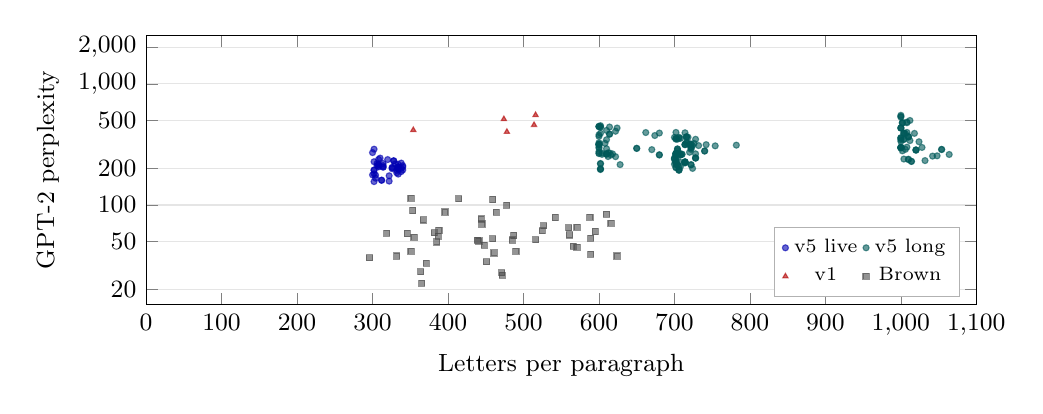
\begin{tikzpicture}
\begin{axis}[
  width=\columnwidth, height=5.0cm,
  ymode=log, log basis y=10, ytick={20,50,100,200,500,1000,2000}, log ticks with fixed point,
  xlabel={Letters per paragraph}, ylabel={GPT-2 perplexity},
  label style={font=\small}, tick label style={font=\small},
  xmin=0, xmax=1100, ymin=15, ymax=2500,
  ymajorgrids, grid style={black!10},
  legend style={font=\scriptsize, at={(0.98,0.03)}, anchor=south east, draw=black!30, legend columns=2},
]
\addplot[only marks, mark=*, mark size=1.1pt, cLive, opacity=0.6] coordinates {(304,166.4) (340,211) (308,208.8) (300,177.2) (302,227.4) (304,176.4) (314,205.3) (340,194.5) (308,237.7) (308,215.8) (308,215.8) (302,194.1) (326,203.6) (328,231.4) (306,220.1) (322,157.3) (338,200.1) (330,218.3) (302,155.9) (300,270.5) (332,192.7) (320,236.9) (306,211.5) (332,184.4) (326,203.6) (302,288.7) (322,174.1) (334,205.3) (334,179.8) (312,160) (308,206.2) (326,199.1) (334,198.2) (302,194.1) (334,198.2) (338,188.6) (314,205.3) (310,243.6) (334,205.3) (334,205.3) (312,160) (302,180.5) (340,205.8) (328,231.4) (314,211.3) (338,221.5) (314,219.7) (334,198.2) (334,198.2) (334,216.5)};
\addlegendentry{v5 live}
\addplot[only marks, mark=*, mark size=1.1pt, cLong, opacity=0.6] coordinates {(704,266.3) (706,268.8) (728,264.3) (702,234.7) (702,233.2) (706,228) (714,314) (714,316) (714,316.3) (704,349) (702,349) (702,352.8) (722,302.3) (722,295.6) (722,296.3) (740,278.7) (722,287.7) (740,278.9) (702,396.9) (714,394.2) (700,361.3) (728,348.3) (716,364) (718,362.2) (754,307.5) (720,320.9) (742,314.5) (700,243) (700,238.2) (700,243.3) (710,261.1) (710,262.9) (720,272.1) (704,289.5) (704,290) (704,281.8) (706,362) (716,365.4) (716,363.6) (702,355.4) (706,355.8) (708,354.5) (720,313.9) (716,328) (716,325.1) (728,243.4) (728,245) (728,244) (704,213.3) (704,214) (700,217.2) (702,262.4) (702,263.2) (704,261.9) (722,317.1) (722,314.5) (724,309) (714,227.1) (702,226.7) (714,225.3) (726,322.3) (782,311.6) (732,309.1) (708,260.1) (708,260.8) (708,257.9) (702,256.3) (702,265.2) (702,263.7) (714,224) (702,223.8) (714,222.2) (702,266.4) (702,267.2) (702,258.3) (714,227.1) (702,226.7) (714,225.3) (706,205.9) (702,204.2) (702,203.1) (702,217.8) (724,200.3) (708,207.5) (706,193.3) (706,194) (706,196.3) (702,223.6) (722,214) (722,215.3) (608,322.9) (610,345.5) (600,325.6) (610,412.4) (614,383.2) (614,385.1) (662,396) (674,374.3) (680,392.3) (680,259.7) (680,258.3) (600,295.1) (604,268.3) (600,275.8) (610,291.3) (602,219.9) (628,215.3) (602,218.7) (1054,287.5) (1054,286.8) (1008,299.9) (1002,279.6) (1000,296.4) (1006,287.6) (1010,367.9) (1010,364.5) (1010,363.6) (1008,477.1) (1008,483) (1012,498.1) (1020,284.6) (1020,283.4) (1020,284.1) (1032,232.4) (1014,228.8) (1014,229.1) (624,431.6) (614,439.8) (622,405.9) (650,293.5) (670,286.2) (650,292.9) (610,263.2) (610,262.8) (610,263.1) (612,250.9) (612,269.1) (616,258.4) (618,264) (614,268.9) (622,250.3) (602,197.8) (602,198.7) (602,196.3) (1012,339.6) (1024,332.4) (1000,335.2) (1006,388.7) (1018,389.9) (1008,397) (1042,253) (1048,254.3) (1064,261) (1000,296.5) (1000,299.8) (1000,298.8) (1000,297) (1000,297.3) (1028,298.4) (1010,236.8) (1004,239.3) (1010,238.6) (600,444.6) (600,443.4) (600,444.2) (602,442.5) (602,437.2) (602,451.5) (600,379.2) (600,368.1) (602,390.5) (600,301.3) (600,313.1) (600,318) (600,315.7) (600,315.9) (600,316) (600,265.5) (604,261.6) (600,268.1) (1002,472.9) (1002,477.6) (1002,479.5) (1000,531.7) (1000,537.7) (1000,549.3) (1000,431.2) (1000,431.9) (1000,432.5) (1004,390.3) (1004,391.4) (1004,391.9) (1000,344.7) (1004,347.1) (1000,352.5) (1000,358.7) (1004,348.8) (1000,358.1)};
\addlegendentry{v5 long}
\addplot[only marks, mark=triangle*, mark size=1.1pt, cvOne, opacity=0.6] coordinates {(478,401.3) (354,415.4) (514,457.3) (474,511.2) (516,552.5)};
\addlegendentry{v1}
\addplot[only marks, mark=square*, mark size=1.1pt, cBrown, opacity=0.6] coordinates {(448,46.5) (595,60.39) (353,89.99) (589,53.16) (371,33.1) (439,51.09) (516,51.49) (472,26.25) (527,67.27) (441,50.38) (319,58.18) (459,52.76) (624,37.84) (478,99.05) (367,75.26) (560,64.72) (485,51.34) (561,56.53) (461,40.18) (444,76.56) (396,87.44) (487,55.93) (414,112.2) (387,55.01) (385,49.49) (471,27.53) (382,59.17) (364,28.19) (296,36.74) (589,39.16) (571,44.83) (355,54.22) (351,113.7) (490,41.51) (332,37.87) (346,58.17) (610,83.81) (588,79.22) (571,65.33) (464,87.09) (525,61.36) (566,45.49) (459,110.9) (365,22.57) (445,69.58) (451,33.92) (388,61.95) (542,78.76) (616,70.43) (351,41.56)};
\addlegendentry{Brown}

\end{axis}
\end{tikzpicture}
\caption{GPT-2 perplexity against length. Within the long corpus the rank correlation is $\rho=\spearmanLong$; within the live corpus $\rho=\spearmanLive$.}
\label{fig:length}
\end{figure}

\paragraph{Length.} Within the long corpus, perplexity barely tracks length (Spearman $\rho=\spearmanLong$, Figure~\ref{fig:length}); a 1,000-letter paragraph is not markedly worse than a 600-letter one. The long corpus sits higher than the live one (median \vFiveSophiaPPL{} against \vFiveLivePPL), but it differs in code version, beam, theme and target, so we do not attribute the gap to length. v1 already closed at any length; the property that matters is that v5's per-token quality does not decay as the beam keeps paying debts.

\paragraph{Where it fails.} Appendix~\ref{app:samples} prints the median live and long paragraphs by GPT-2 perplexity. Their sentences are short and many are grammatical in isolation (\w{I hate me. Here are we now to ten or even\dots}); the failures are dangling function words where a debt was paid with whatever fit (\w{as a were held}), and the absence of any thread between sentences. Themes add topical words (\w{stars}, \w{rose}, \w{sea}) without adding a subject that persists.

\section{Proposed human evaluation}\label{sec:human}

No reader has judged v5 in a controlled study, and the automatic results above cannot substitute for one. We will run the following protocol before claiming readability.

\paragraph{Items.} Five conditions at matched length (300--340 letters, or 60--120 words for prose): v5 live; v1; Brown passages; v5 paragraphs with words shuffled within each sentence (salad control that keeps v5's vocabulary and punctuation); and v5 rendered without punctuation or capitals (sizes the presentational share of the GPT-2 gain). Thirty items per condition, drawn by seed before any rating.

\paragraph{Judgements.} Raters, blind to condition and to the palindrome property, rate each sentence for grammaticality (0--3) and each paragraph for meaning (0--3), with written anchors as in our earlier rubric, and answer a pairwise forced choice between v5 and v1 at matched length with position balanced. Each item receives five ratings; attention checks use Brown and shuffled controls with known answers.

\paragraph{Analysis.} Pre-registered hypotheses: (H1) v5 sentences outscore v1 on grammaticality; (H2) v5 does not reach Brown; (H3) the verifier's readability probability correlates with human sentence grammaticality on held-out v5 sentences (Spearman, with a bootstrap interval). H3 is the test the verifier has not had: its AUC was measured against v1 and shuffles, and inside the beam it may be rewarding sentences readers reject. Ordinal mixed-effects models with rater and item intercepts; inter-rater agreement by Krippendorff's $\alpha$.

\section{Discussion}

The four failures and v5 together delimit the design space. Text cannot be scored only on the half the search can see (v1), cannot be borrowed (v2), cannot be assembled from units that are palindromes on their own (v3), and cannot be forced through a small set of grammatical frames (v4). What remains is a search that lets the two halves disagree about word and sentence boundaries, scores both with a model of ordinary prose as they grow, and judges each sentence as it closes. v5 is that search. Its outputs are exact at any length we have tried, beat the earlier word-level search by a wide margin on an independent model, and remain far from prose.

Three directions follow from the measurements. The short-word share is the clearest target, since v5 is worse than v1 on it: a cost on one- and two-letter debts, or a lexicon that prefers longer exact fits, attacks it directly. Themes cut cross-run overlap by a factor of four; a penalty on recently emitted phrases would attack the chains that survive them. And the verifier should be retrained once human judgements of v5 sentences exist, because a scorer fitted to reject v1 is now saturated by the generator it steers.

\section*{Limitations}
The verifier and the trigram model are both objective and measurement; Table~\ref{tab:main} marks every such row, and none of them is evidence that v5 reads well. GPT-2 perplexity is independent of the search but is a fluency proxy, rewards punctuation and capitals that v1 lacks, and has not been validated against readers on palindromic text. No human study has been run on v5. The v1 comparison corpus has \vOneN{} outputs but only \vOneDistinct{} distinct texts. The long corpus mixes development batches with differing code, beam widths and targets. The verifier's anchors are human forum palindromes, Brown sentences and classics against v1 windows and shuffles; its AUC says nothing about the boundary between v5's sentences and human prose. Brown and Gutenberg text supply the vocabulary and the prose model, so the register is mid-century American and older literary English. The work is English only. Earlier measurements cited from the project's history (v1--v4) come from different evaluation setups and are not directly comparable with each other or with Table~\ref{tab:main}.

\section*{Ethical considerations}
No human participants were involved. The training corpora are public; the human palindromes used as verifier anchors are short public posts used only as feature-fitting data and are not reproduced. Model scores are never presented as human judgements. Generative AI assisted with implementation and writing.

\bibliography{references}

\appendix

\section{Settings}\label{app:settings}
\begin{table}[h]
\centering\small
\begin{tabular}{@{}l r@{}}
\toprule
Parameter & Production \\
\midrule
Target letters / slack & 300 / 40 \\
Beam width / children per parent & 200 / 12 \\
LM-ranked candidates per debt & 30 \\
Overrun candidates per debt (by frequency) & 150 \\
Maximum debt (letters) & 8 \\
Priority: per letter / per owed letter & 0.7 / 0.4 \\
Sentence weight / comma cost & 2.0 / 1.0 \\
Content bonus / local / far repeat & 1.6 / 4.0 / 0.5 \\
Near-window repeat / cycle & 4.0 / 6.0 \\
Run-on window (tokens) / cost per word & 18 / 2.0 \\
Seam-insert cost & 1.0 \\
Theme weight (first use) & 15 \\
Start noise / steps; later noise & 4.0 / 8; 0.3 \\
Lexicon minimum count & 3 \\
\bottomrule
\end{tabular}
\caption{Settings of the deployed generator.}
\end{table}

The lexicon keeps alphabetic words seen at least three times in the prose corpus that are attested in Brown other than as proper nouns, excluding contraction stems (\w{didn}, \w{wouldn}) and words of one or two letters outside an allowlist of real short words. The left half is scored by the same forward model as the right; a hook for periodic re-scoring by a neural model exists in the code and is disabled in production, so no neural model is in v5's loop.

\section{Sample outputs}\label{app:samples}
\paragraph{v5 live, median GPT-2 perplexity (314 letters).}
\small
\begin{quote}
Till at last, are here may be not I won kill it never even a man. I put new era. Consider it to get on a net for ever. Of no part nor in all am so still. If I did not at all a cotton field is it I saw one man went on, not new name. Now, as it is idle. If not to call at a ton. Did I fill it. So small an iron trap on forever. Often, a note. Got tired is no care went up in a man ever, even till I know it. One by a mere her at salt. All. It.
\end{quote}
\normalsize
\paragraph{v5 long, lowest GPT-2 perplexity (706 letters, theme not shown), first half.}
\small
\begin{quote}
Sun, or of stars. I hate me help missiles. Seven of iron are hosts. A foot too fat ones. I arise. Yes, till it was a fine my bed. I say as to no die not satisfied is still a walk said neon sign. I care not for one year of never even a month girl late so temple hosts. It ran as a tired. Now I met in it for ever. Of evil, as I lived an idle. His eye, yet so may be no part nor in all I know it. \dots
\end{quote}
\normalsize

\end{document}
